\documentclass{article}

% Paquetes comunes
\usepackage[utf8]{inputenc}
\usepackage[T1]{fontenc}
\usepackage[spanish]{babel}
\usepackage{amsmath, amssymb}
\usepackage{graphicx}
\usepackage{float}
\usepackage{geometry}
\usepackage{hyperref}
\usepackage{fancyhdr}
\usepackage{textcomp}
\usepackage{circuitikz}
% Saltar entre párrafos - sin sangrías
\usepackage{parskip}

% Márgenes
\geometry{a4paper, margin=2.5cm}

% Encabezado y pie de página
\pagestyle{fancy}
\fancyhf{}
\fancyhead[L]{\textbf{Tarea 4} - Tomas Infante}
\fancyhead[R]{IEE2513}
\fancyfoot[C]{\thepage}

\title{Tarea 4}
\author{Tomas Infante}
\date{\today}
\begin{document}
\begin{figure}[H]
    \centering
    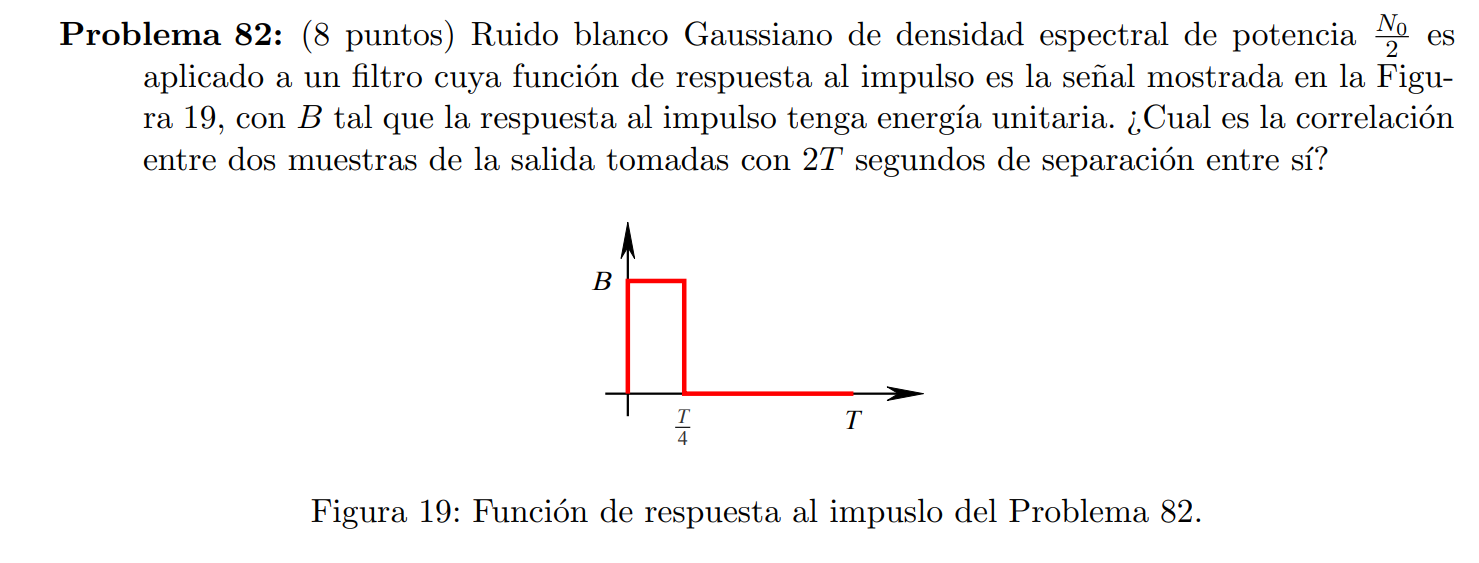
\includegraphics[width=1\textwidth]{Problema_82.png}
    \label{Problema_82}
\end{figure}
Vemos que a partir de la grafica podemos definir la respuesta al impulso del filtro como:
\[
h(t)=
\begin{cases}
B, & 0 \le t \le \frac{T}{4} \\[6pt]
0, & \text{en otro caso}
\end{cases}
\]
Por otra parte nos dice el enunciado que la respuesta al impulso tiene que tener energia unitaria. Es decir:
\[
\int_{-\infty}^{\infty}|h(t)|^{2}\,dt = 1
\]
Por como esta definido \(h(t)\) tenemos que la expresiona anterior se reduce a:
\[
\int_{0}^{\frac{T}{4}}B^{2}\,dt = 1
\]
Resolvemos y llegamos a:
\[
B^{2}\left(\frac{T}{4}\right)=1 \quad \longrightarrow \quad B=\pm\frac{2}{\sqrt{T}}
\]
Como evidentemente \(B>0\) tomamos el valor positivo.\\

Definimos la salida del filtro como:
\[
y(t) = h(t)\ast x(t) \quad \longrightarrow \quad y(t) = \int_{-\infty}^{\infty}h(\tau)x(\tau-t)\,dt
\]
Donde \(x(t)\) es la entrada al filtro, \(h(t)\) la respuesta al impulso del filtro y \(y(t)\) la salida del filtro. \\

El enunciado nos pide calcular la correlacion entre 2 muestras de la salida tomadas con \(2T\) segundos de separacion. Como el ruido blanco gaussiano es ESA entonces tambien lo es \(y(t)\), lo que reduce el probelma a simplemente calcular:
\[
R_y(2T) = E\left[y(t)y(t+2T)\right]
\]
\[
R_y(2T) = E\left[\left(\int_{-\infty}^{\infty}h(\tau_1)x(\tau_1-t)\,d\tau_1\right) \left(\int_{-\infty}^{\infty}h(\tau_2)x(\tau_2-(t+2T))\,d\tau_2\right)\right]
\]
Usamos propiedades de la esperanza, para meterla dentro de la integral y sacar \(h\) fuera de la esperanza ya que no es aleatoria.
\[
R_y(2T) = \int_{-\infty}^{\infty}\int_{-\infty}^{\infty}h(\tau_1)h(\tau_2)E\left[x(\tau_1-t) x(\tau_2-(t+2T))\right]\,d\tau_1\,d\tau_2
\]
Como \(x(t)\) es ruido blanco gaussiano sabemos que su funcion de autocorrelacion se ve como:
\[
R_x(\tau) = \frac{N_0}{2}\delta(\tau)
\]
Y literalmente:
\[
E\left[x(\tau_1-t) x(\tau_2-(t+2T))\right] = R_x(\tau_1-\tau_2 +2T) = \frac{N_0}{2}\delta(\tau_1-\tau_2 +2T)
\]
Reemplzando lo anterior llegamos a:
\[
R_y(2T) = \frac{N_0}{2}\int_{-\infty}^{\infty}\int_{-\infty}^{\infty}h(\tau_1)h(\tau_2)\delta(\tau_1-\tau_2 +2T)\,d\tau_1\,d\tau_2
\]
Debemos resolver alguna integral primero, sea cual sea llegamos al mismo resultado ya que al resolver la primera llegamos, por porpiedades de la funcion delta, a:
\[
R_y(2T) = \frac{N_0}{2}\int_{-\infty}^{\infty}h(\tau_1)h(\tau_1 + 2T)\,d\tau_1
\]
Como \(h(\tau)\neq 0\) solo si \(0\le \tau \le \frac{T}{4}\), y
\(h(\tau+2T)\neq 0\) solo si:
\[
0 \le \tau+2T \le \frac{T}{4}
\;\;\Longrightarrow\;\;
-2T \le \tau \le -\frac{7T}{4},
\]

los intervalos no se intersectan. Por lo tanto,
\[
h(\tau)\,h(\tau+2T)=0 \quad \forall\,\tau,
\]

y así
\[
R_y(2T)=\frac{N_0}{2}\int_{-\infty}^{\infty}0\,d\tau=0.
\]

\[
\boxed{R_y(2T)=0}
\]
\end{document}